% =============================================================================
% 5.5 代码生成与受限沙箱三档消融
% 草稿版本：v0.2 (2026-05-07)
%   v0.1：作为 5.2.4 子小节起草。
%   v0.2：按导师意见 3 提级为 5.5 \subsection。
% 字数：约 1300 字
% 风格规则：v0.2 风格（无 \textbf / \textit / 引例括号 / 双引号 / 破折号）
% 引用：\cite{ref20, ref23, ref29}
% 图表：
%   - 图 \reffig{fig:code-eval-overall}   3 档数值准确率柱状图（含代码生成 / 可执行率）
%   - 图 \reffig{fig:code-eval-category}  6 类用例上 direct vs with_code 双档对比
%   - 表 \reftab{tab:code-fail-modes}     四类典型幻觉模式失败用例统计
% 复用 4.2 节已有图表：
%   - \reftab{tab:code-bench-design}     评测集任务分布
%   - \reftab{tab:code-eval-overall}     3 档总表
%   - \reftab{tab:code-eval-category}    按类别拆分
% 依赖宏包：booktabs / tabularx / graphicx（主稿已加载）
% =============================================================================

\subsection{代码生成与受限沙箱三档消融}
\label{sec:code-eval}

代码生成与受限沙箱的 3 档消融总表已在 \ref{sec:code-execution} 节
\reftab{tab:code-eval-overall} 给出，按类别拆分见
\reftab{tab:code-eval-category}。本节聚焦四件 \ref{sec:code-execution}
节未展开的内容：评测集 18 条用例的设计思路、三档消融的具体差异化设置、
四类失败模式的统计分布、以及大语言模型在多步统计任务上中间状态
维护能力的边界讨论。

评测集 \texttt{code\_\bk{}exec\_\bk{}bench.\bk{}jsonl} 共 18 条用例，覆盖 6 类统计模式
\texttt{average /\bk{} extreme /\bk{} sum /\bk{} diff /\bk{} count /\bk{} sort}。具体任务分布
已在 \reftab{tab:code-bench-design} 给出。每类用例都故意包含若干边界
情形以放大失败概率，例如 \texttt{average} 类含 24.95 的银行家舍入
边界，\texttt{count} 类含 35.0 °C 高温阈值平等，\texttt{sum} 类含
仅高温日的条件累计降水。每条用例标注 \texttt{expected.\bk{}value} 与
\texttt{tolerance} 容差，并按答案结构分为 \texttt{scalar /\bk{} date /\bk{}
date\_\bk{}with\_\bk{}value /\bk{} time\_\bk{}with\_\bk{}value /\bk{} ordered\_\bk{}list} 五种类型。
其中 4 条 \texttt{*\_\bk{}with\_\bk{}value} 类型要求模型同时给出哪一天与对应
数值，是评测中刻意设计的复合答案压力测试。

三档消融的具体差异化设置如下。\texttt{oracle} 档直接读取
\texttt{expected.\bk{}value} 作为输出，作为评测器自校验天花板，确认比较
函数本身的正确性，结果数值准确率 100.0\%。\texttt{llm\_\bk{}direct} 档
向模型同时提供查询语句与数据样例，但 prompt 显式禁止生成代码，要求
直接给出 \texttt{value} 字段。这一档作为大语言模型自由发挥的对照。
\texttt{llm\_\bk{}with\_\bk{}code} 档让模型在 function calling 模式下生成
\texttt{compute(data)} 顶层函数，函数代码送入 \texttt{src/\bk{}tools/\bk{}code\_\bk{}executor.\bk{}py}
受限沙箱执行后，取沙箱返回值作为最终答案。三档使用同一被测模型
GLM-5.1，避免引入模型差异。\texttt{llm\_\bk{}direct} 档数值准确率为 66.7\%，
\texttt{llm\_\bk{}with\_\bk{}code} 档为 88.9\%，差距 22.2 个百分点。代码生成率
与代码可执行率均为 94.4\%，证明模型在 function calling 下生成可执行
代码的能力是稳定的，失败主要来自单条用例上的算法或字段命名错误，而
非工具调用基础能力。三档对比的整体走势见
\reffig{fig:code-eval-overall}。

\begin{figure}[!ht]
    \centering
    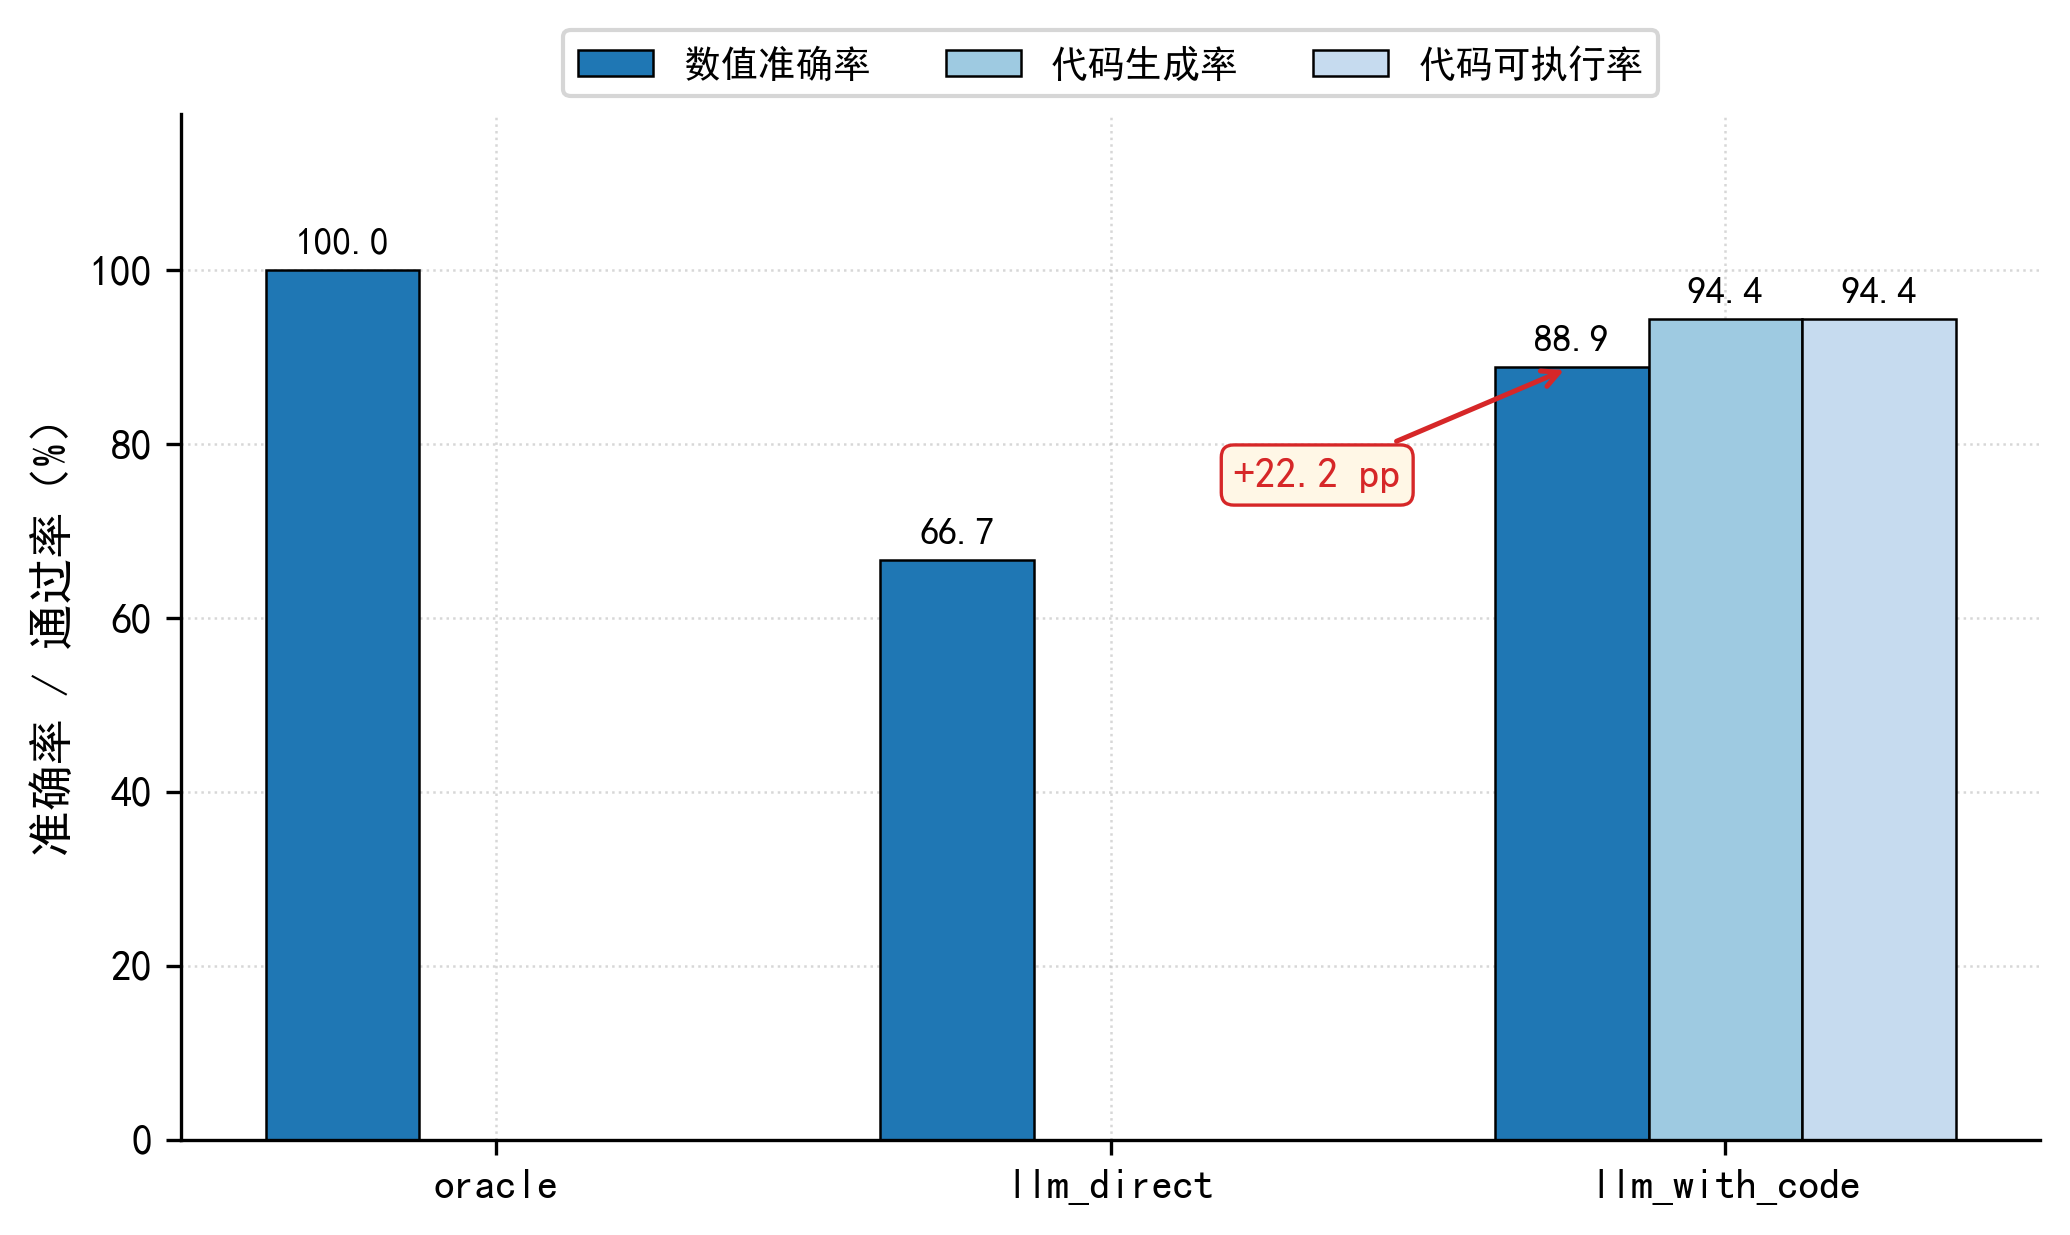
\includegraphics[width=0.78\linewidth]{figures/eval_5_3_code_overall}
    \caption{代码执行三档总体对比：数值准确率与代码生成 / 可执行率（18 条评测集）}
    \label{fig:code-eval-overall}
\end{figure}

按类别拆分的差距分布揭示了大语言模型直算的能力边界规律，详见
\reftab{tab:code-eval-category} 与 \reffig{fig:code-eval-category}。差距最大的两类是极值与计数：
\texttt{extreme} 类 \texttt{llm\_\bk{}direct} 准确率为 0.0\%，三条全部
失败；\texttt{count} 类 \texttt{llm\_\bk{}direct} 准确率仅 50.0\%。差距
最小的两类是求和与排序：两档都达到 100.0\%。简单求和与天然排序任务
不需要伴随状态维护或离散计数，模型凭语料能力可以做对；但只要任务
需要在找最大值的同时记录对应日期等伴随状态，或需要离散累加器，模型
就会犯错。这一规律可以直观理解为：模型在不需要维护中间状态的简单
计算上能够依靠语料能力给出正确答案，而一旦任务需要持续跟踪中间
结果就容易出错。同样的工程取舍也可见于 Hong 等 \cite{ref20} 在
Data Interpreter 中的设计思路，将多步数据科学任务交由代码执行
而非纯 prompt 推理来完成，以回避模型在中间状态维护上的局限。代码
执行的本质即是给模型配上一支笔与一张草稿纸，把心算换成笔算。

\begin{figure}[!ht]
    \centering
    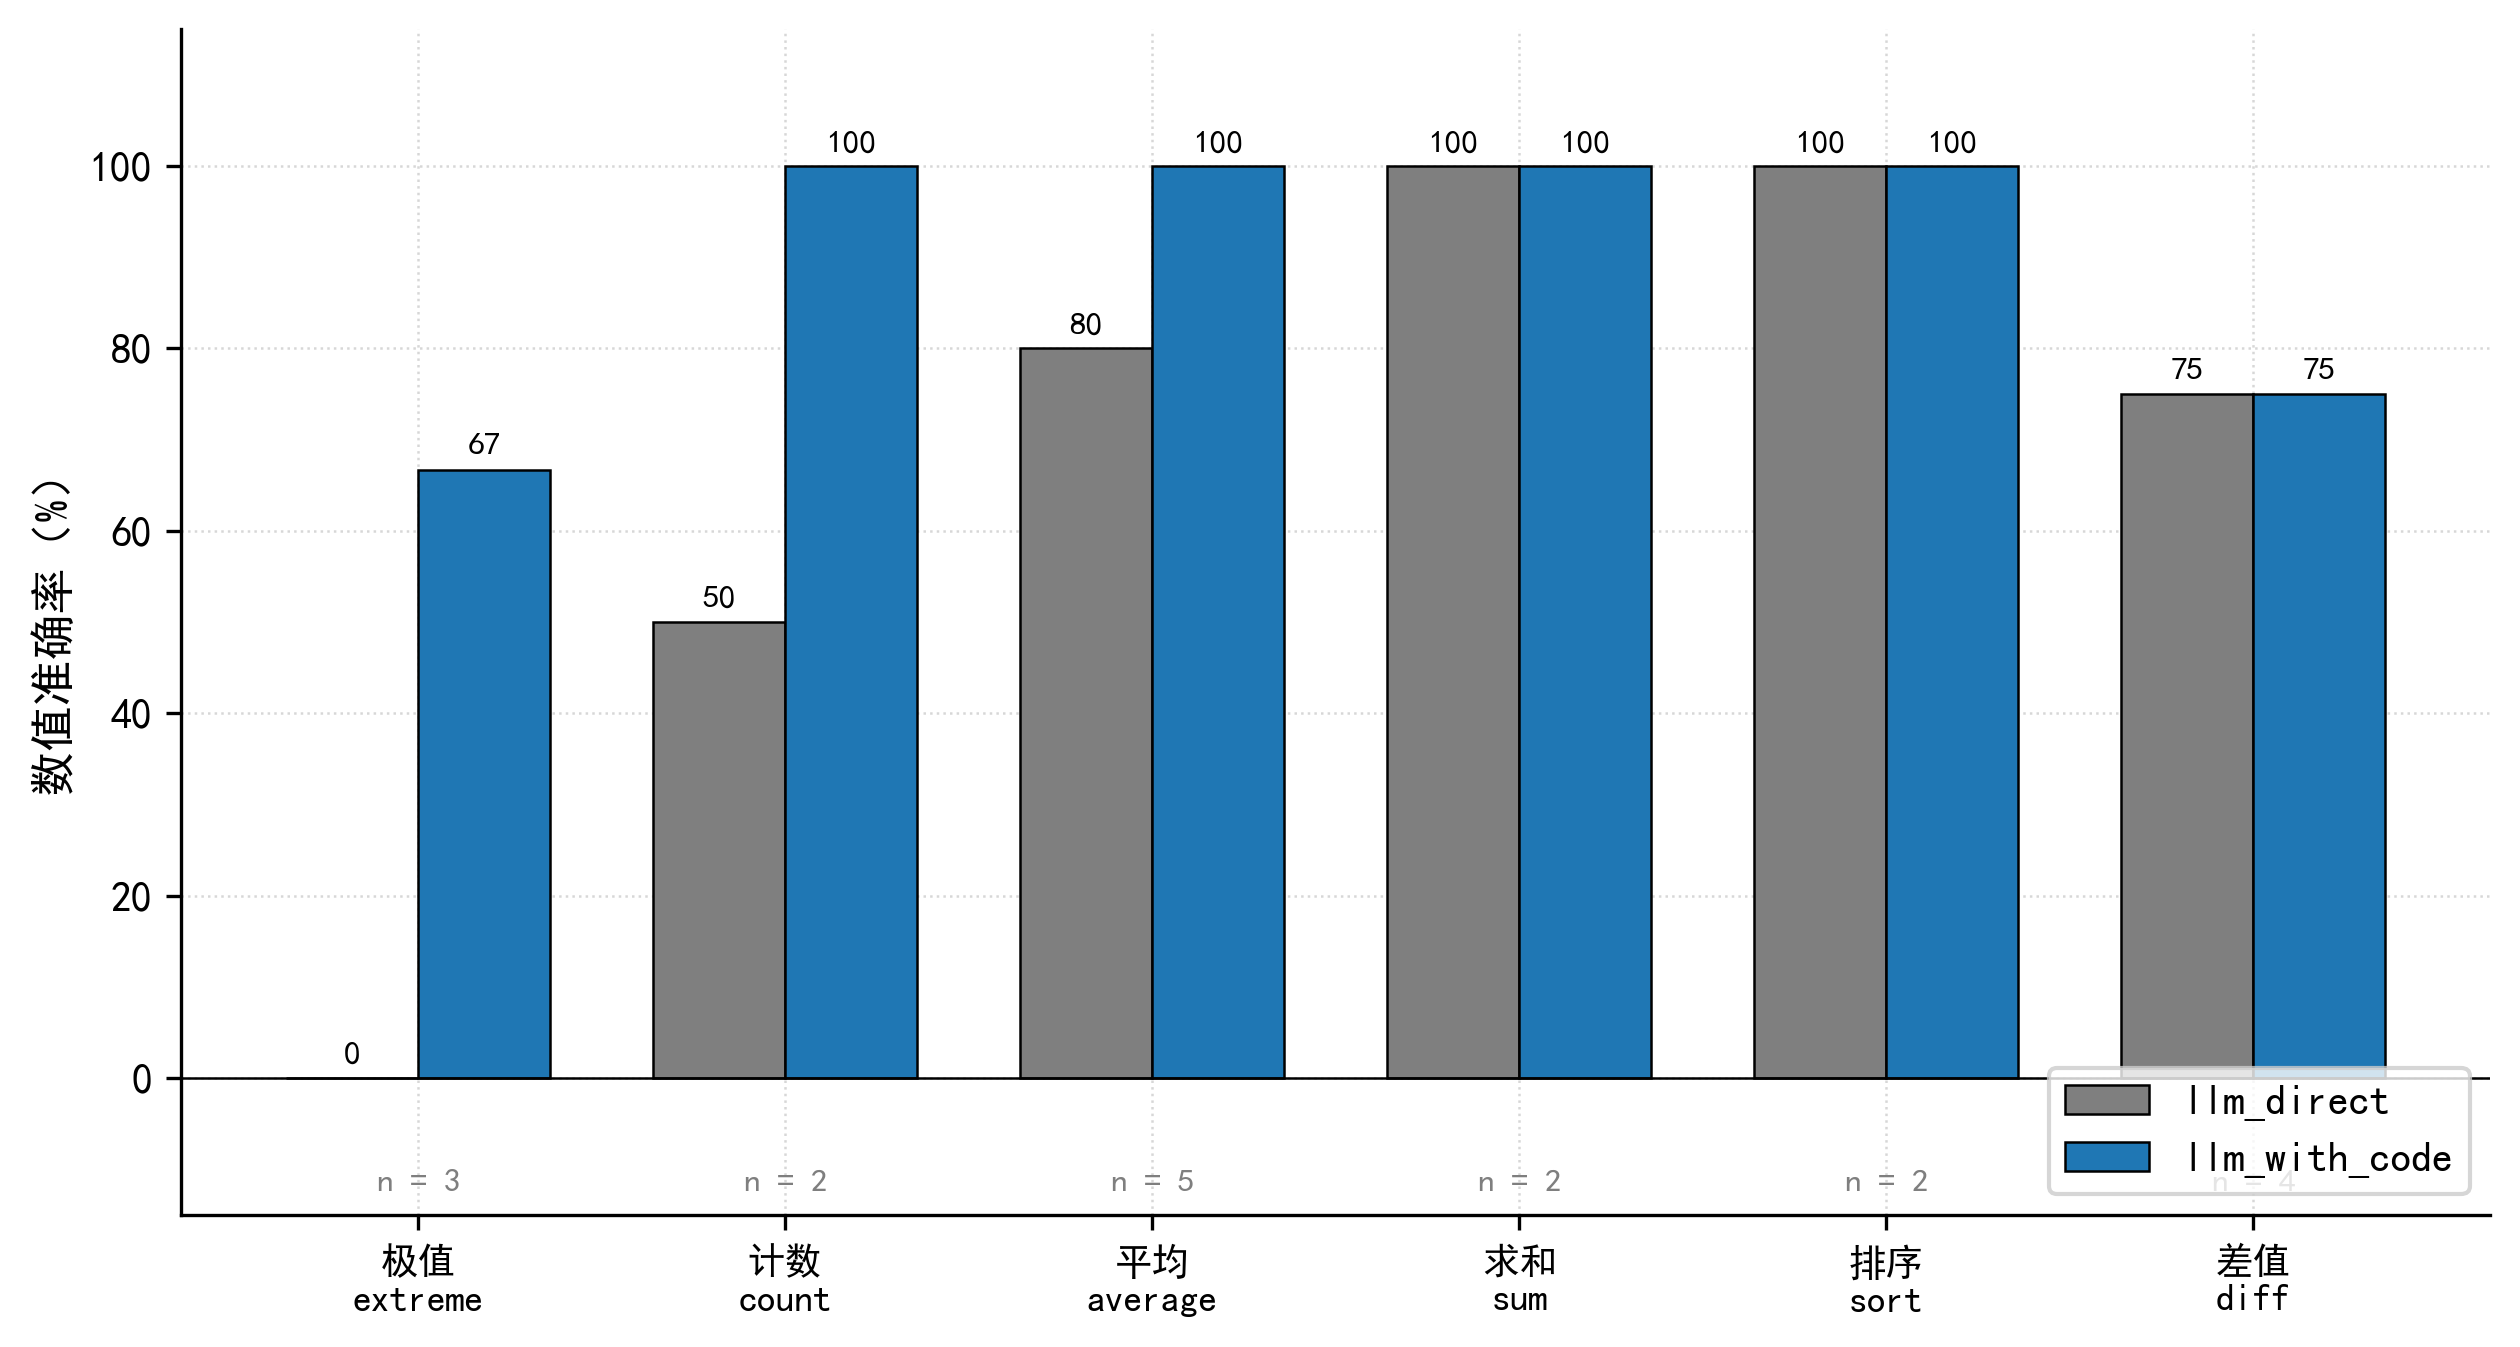
\includegraphics[width=0.92\linewidth]{figures/eval_5_4_code_by_category}
    \caption{代码执行按用例类别拆分：\texttt{llm\_direct} 与 \texttt{llm\_with\_code} 在 6 类统计模式上的数值准确率对比}
    \label{fig:code-eval-category}
\end{figure}

逐条分析 \texttt{llm\_\bk{}direct} 档 6 条失败用例与 \texttt{llm\_\bk{}with\_\bk{}code}
档 2 条失败用例，可归纳出四类典型幻觉模式，分布见
\reftab{tab:code-fail-modes}。

\begin{table}[H]
    \centering
    \caption{代码执行评测四类典型失败模式分布}
    \label{tab:code-fail-modes}
    \song\fontsize{9pt}{12pt}\selectfont
    \renewcommand{\arraystretch}{0.95}
    \begin{tabular}{llcc}
        \toprule
        失败模式 & 代表用例 & llm\_direct & llm\_with\_code \\
        \midrule
        数数错误（reasoning 自相矛盾） & \texttt{count\_\bk{}001\_\bk{}rainy\_\bk{}days} & 1 & 0 \\
        舍入不一致（教科书 vs 银行家） & \texttt{avg\_\bk{}005\_\bk{}feels\_\bk{}like} & 1 & 0 \\
        Schema 不稳定（复合答案被压扁） & \texttt{extreme\_001 \textasciitilde{} 003}, \texttt{diff\_\bk{}001} & 4 & 1 \\
        字段命名漂移（range 与 tempDiff） & \texttt{diff\_\bk{}001\_\bk{}max\_\bk{}diurnal} & 0 & 1 \\
        \midrule
        \multicolumn{2}{c}{合计失败用例数} & 6 & 2 \\
        \bottomrule
    \end{tabular}
\end{table}

第一类数数错误的危险性最高。\texttt{count\_\bk{}001\_\bk{}rainy\_\bk{}days} 用例
要求统计 14 天中降水量大于 0 的天数，正确答案为 7。模型在
\texttt{reasoning} 字段中正确列举了 7 个具体日期，但 \texttt{value}
字段却给出了 6。推理过程与最终答案的自相矛盾意味着即便用户阅读
\texttt{reasoning} 也会被说服，难以察觉数值错误。代码档对照仅需一行
\texttt{sum(1 for d in daily if d["precip"] > 0)} 即可正确返回 7。

第二类舍入不一致体现的是语境敏感型精度幻觉。\texttt{avg\_\bk{}005\_\bk{}feels\_\bk{}like}
用例的精确均值为 24.95，使用 Python 标准 \texttt{round} 函数即 IEEE 754
银行家舍入向偶数舍入应得 24.9。模型给出 25.0 并在 reasoning 中说明
按四舍五入保留 1 位小数，反映其默认采用中学教科书规则。在工程数据
处理上下文中下游所有数值处理都默认使用 Python 标准舍入，这种语义
偏移在工程接管中是不可接受的。

第三类 schema 不稳定是占比最大的失败模式。\texttt{extreme\_\bk{}001} 至
\texttt{extreme\_\bk{}003} 与 \texttt{diff\_\bk{}001} 共 4 条 \texttt{llm\_\bk{}direct}
失败用例都属于这一类。Prompt 已经显式约定把日期放在 \texttt{value}
字段、把数值放在 \texttt{numeric\_\bk{}extra} 字段，但模型在 function
calling 下仍只填日期字段而把数值留作自由文本。这一现象与本文通路 B
评测中模型不稳定遵循 \texttt{grade\_\bk{}id} 命名约定的观察相互印证：
结构化输出的可靠性随 schema 复杂度上升而急剧下降是大语言模型应用
工程中的经典痛点。

第四类字段命名漂移仅出现在 \texttt{llm\_\bk{}with\_\bk{}code} 档的
\texttt{diff\_\bk{}001} 用例。生成代码逻辑完全正确，找出温差最大的
2025-09-18 一天，温差 22.7 摄氏度，但返回字典字段名为 \texttt{range}
而非期望的 \texttt{tempDiff}。这一类失败可以通过更严格的 schema 约束
或下游适配层缓解，与算法能力无关。

需要明确的是，本文设计的沙箱属于轻量原型，主动放弃了完整的安全隔离。
真实生产环境下应当使用 RestrictedPython、Pyodide 或 Docker 容器实现
进程级隔离；像 Boiko 等 \cite{ref23} 在 Coscientist 中将代码执行与
真实化学实验设备直接耦合的科研场景对沙箱安全的要求更为严格。完整
的安全沙箱方案在 \ref{sec:future-work} 节作为未来工作展开。
